%!TEX root = ../terrainbook.tex

\graphicspath{{interpol/}}

\chapter{Spatial interpolation: polynomials and weighted-average methods}%
\label{chap:interpol}


% \chaptertoc

Given a set $S$ of points $p_i$ in $\mathbb{R}^2$ (also called samples or data points in the following) to which an attribute $a_i$ is attached, spatial interpolation is the procedure used to estimate the value of the attribute at an unsampled location $x$. 
Its goal is to find a function $f(x,y)$ that fits (pass through, or close to, all the points in $S$) as well as possible. 
There is an infinity of such functions, some are global and some are piecewise, an thus we the aim is to find one that is best suited for the kind of datasets used as input.
Interpolation is based on \emph{spatial autocorrelation}, that is the attribute of two points close together in space is more likely to be similar than that of two points far from each other.

%

It should be noticed that the natural spatial extent of a set of sample is its \emph{convex hull}, and that an estimation outside this convex hull is \emph{extrapolation}.
\begin{figure}
  \centering
  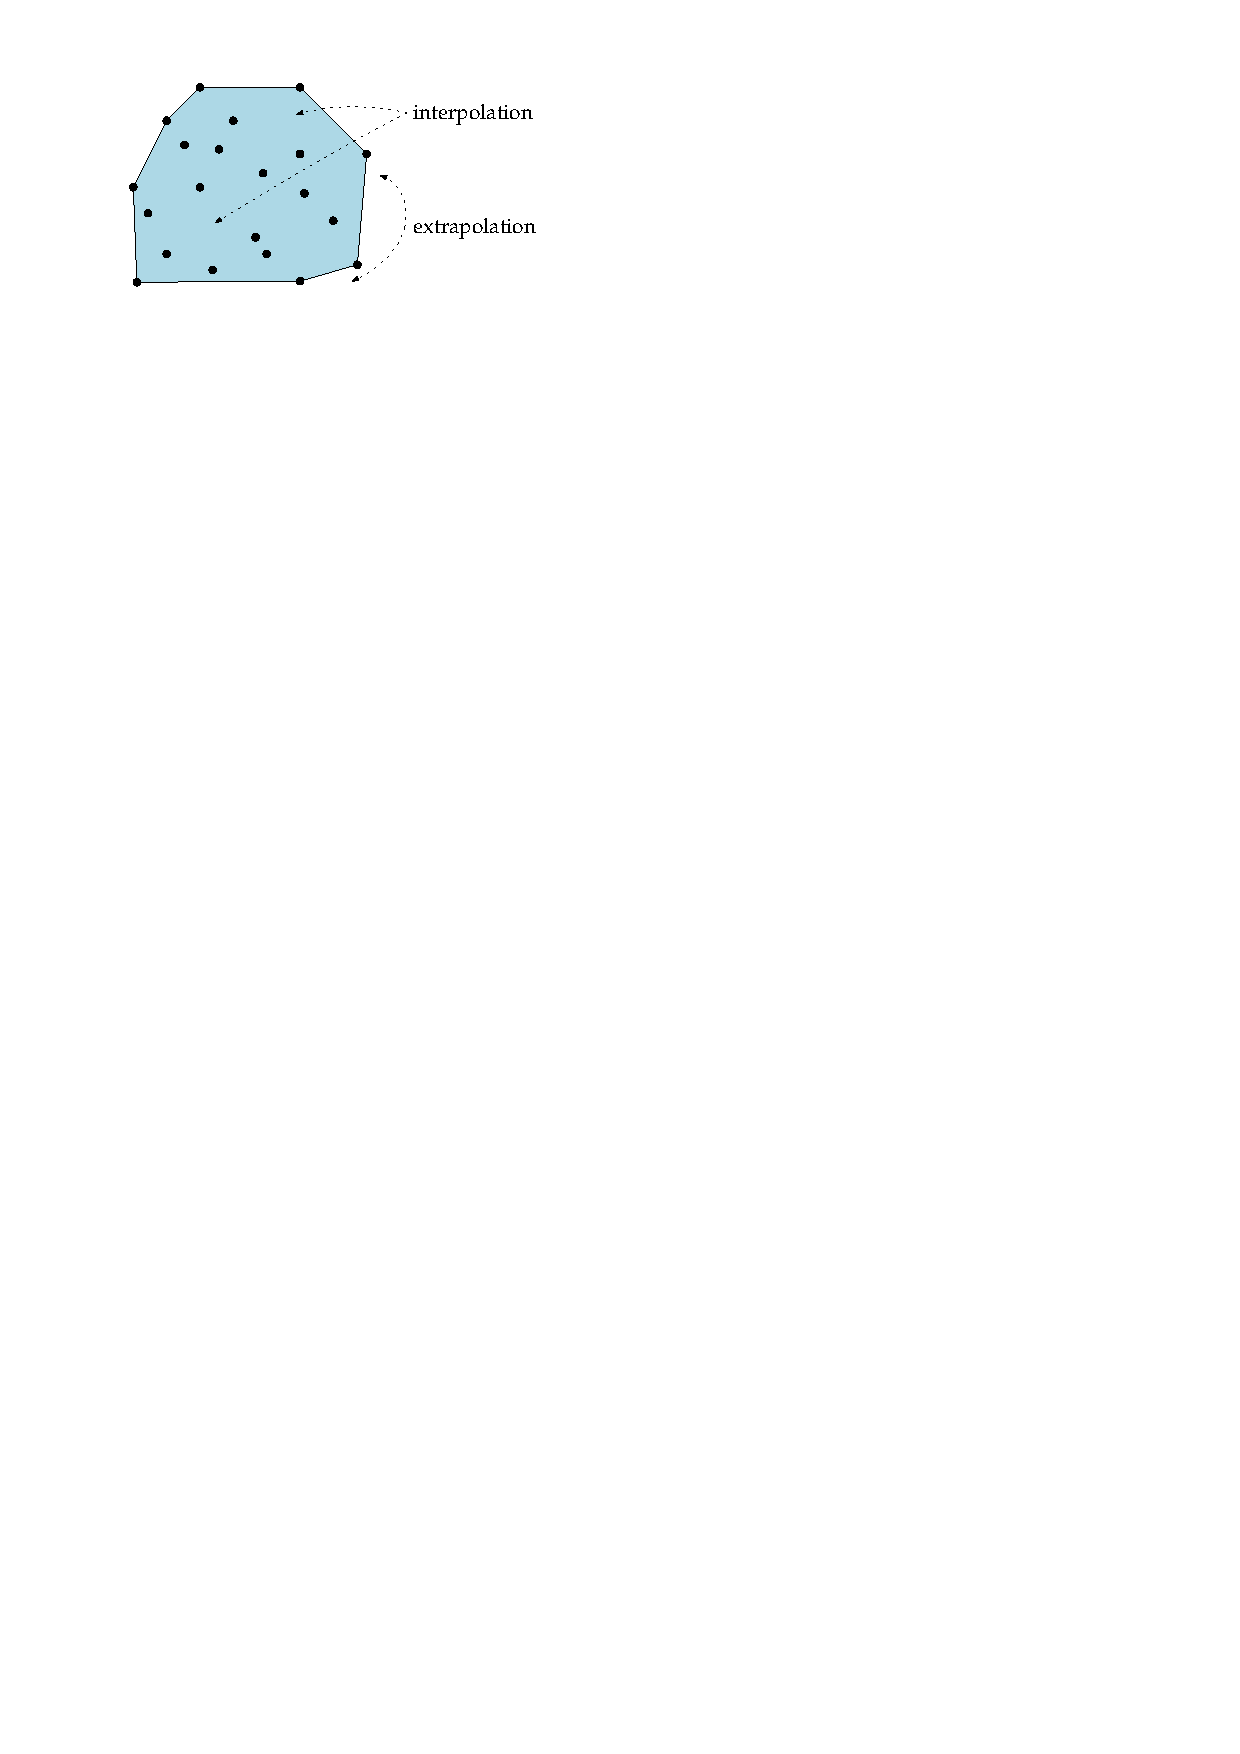
\includegraphics[width=0.4\linewidth]{figs/extrapolation}
  \caption{Spatial interpolation and extrapolation.}
\label{fig:extrapolation}
\end{figure}
Extrapolating implies that more uncertainty is attached to the estimated value.

%

Spatial interpolation methods are crucial in the visualisation process (\eg\ generation of contours lines), for the conversion of data from one format to another (\eg\ from scattered points to raster), to have a better understanding of a dataset, or simply to identify `bad' samples. 
The result of interpolation---usually a surface that represents the terrain---must be as accurate as possible because it often forms the basis for spatial analysis, for example runoff modelling or visibility analysis. 
Although interpolation helps in creating three-dimensional surfaces, in the case of terrains it is intrinsically a two-dimensional operation because only the ($x,y$) coordinates of each sample are used, and the elevation is the dependent attribute.
Notice that the attribute used need not be only elevation, for other GIS applications one could use the spatial interpolation methods below for for instance rainfall amounts, percentage of humidity in the soil, maximum temperature, etc. 
Spatial interpolation in 3D is also possible (but out of scope for this course), in that case there are 3 independent variables ($x,y,z$) and one dependent variable, for instance the temperature of the sea at different depth, or the concentration of a certain chemical in the ground.


%


%-------------------------------------------------
%%%
\section{What is a good interpolation method for terrains?}

The essential properties of an `ideal' interpolation method for bivariate geoscientific datasets are as follows:
\begin{enumerate}
  \item \textbf{exact}: the interpolant must `honour' the data points, or `pass through' them.
  \item \textbf{continuous}: a single and unique value must be obtained at each location. This is called a $C^0$ interpolant in mathematics (see Figure~\ref{fig:continuity}).
  \item \textbf{smooth}: it is desirable for some applications to have a function for which the first or second derivative is possible everywhere; such functions are respectively referred to as $C^1$ and $C^2$ interpolants.
  \item \textbf{local}: the interpolation function uses only some neighbouring samples to estimate the value at a given location. This ensures that a sample with a gross error will not propagate its error to the whole interpolant.
  \item \textbf{adaptability}: the function should give realistic results for anisotropic data distributions and/or for datasets where the data density varies greatly from one location to another.
  \item \textbf{computationally efficient}: it should be possible to implement the method and get an efficient result. Efficient is of course subjective. For a student doing this course, efficiency might mean that the method generates a result in matter of minutes or an hour on a laptop, for the homework dataset. For a mapping agency, running a process for a day on a supercomputer for a whole country might be efficient.
  \item \textbf{automatic}: the method must require as little input as possible from the user, \ie\ it should not rely on user-defined parameters that require \emph{a priori} knowledge of the dataset.
\end{enumerate}
\begin{figure}
  \centering
  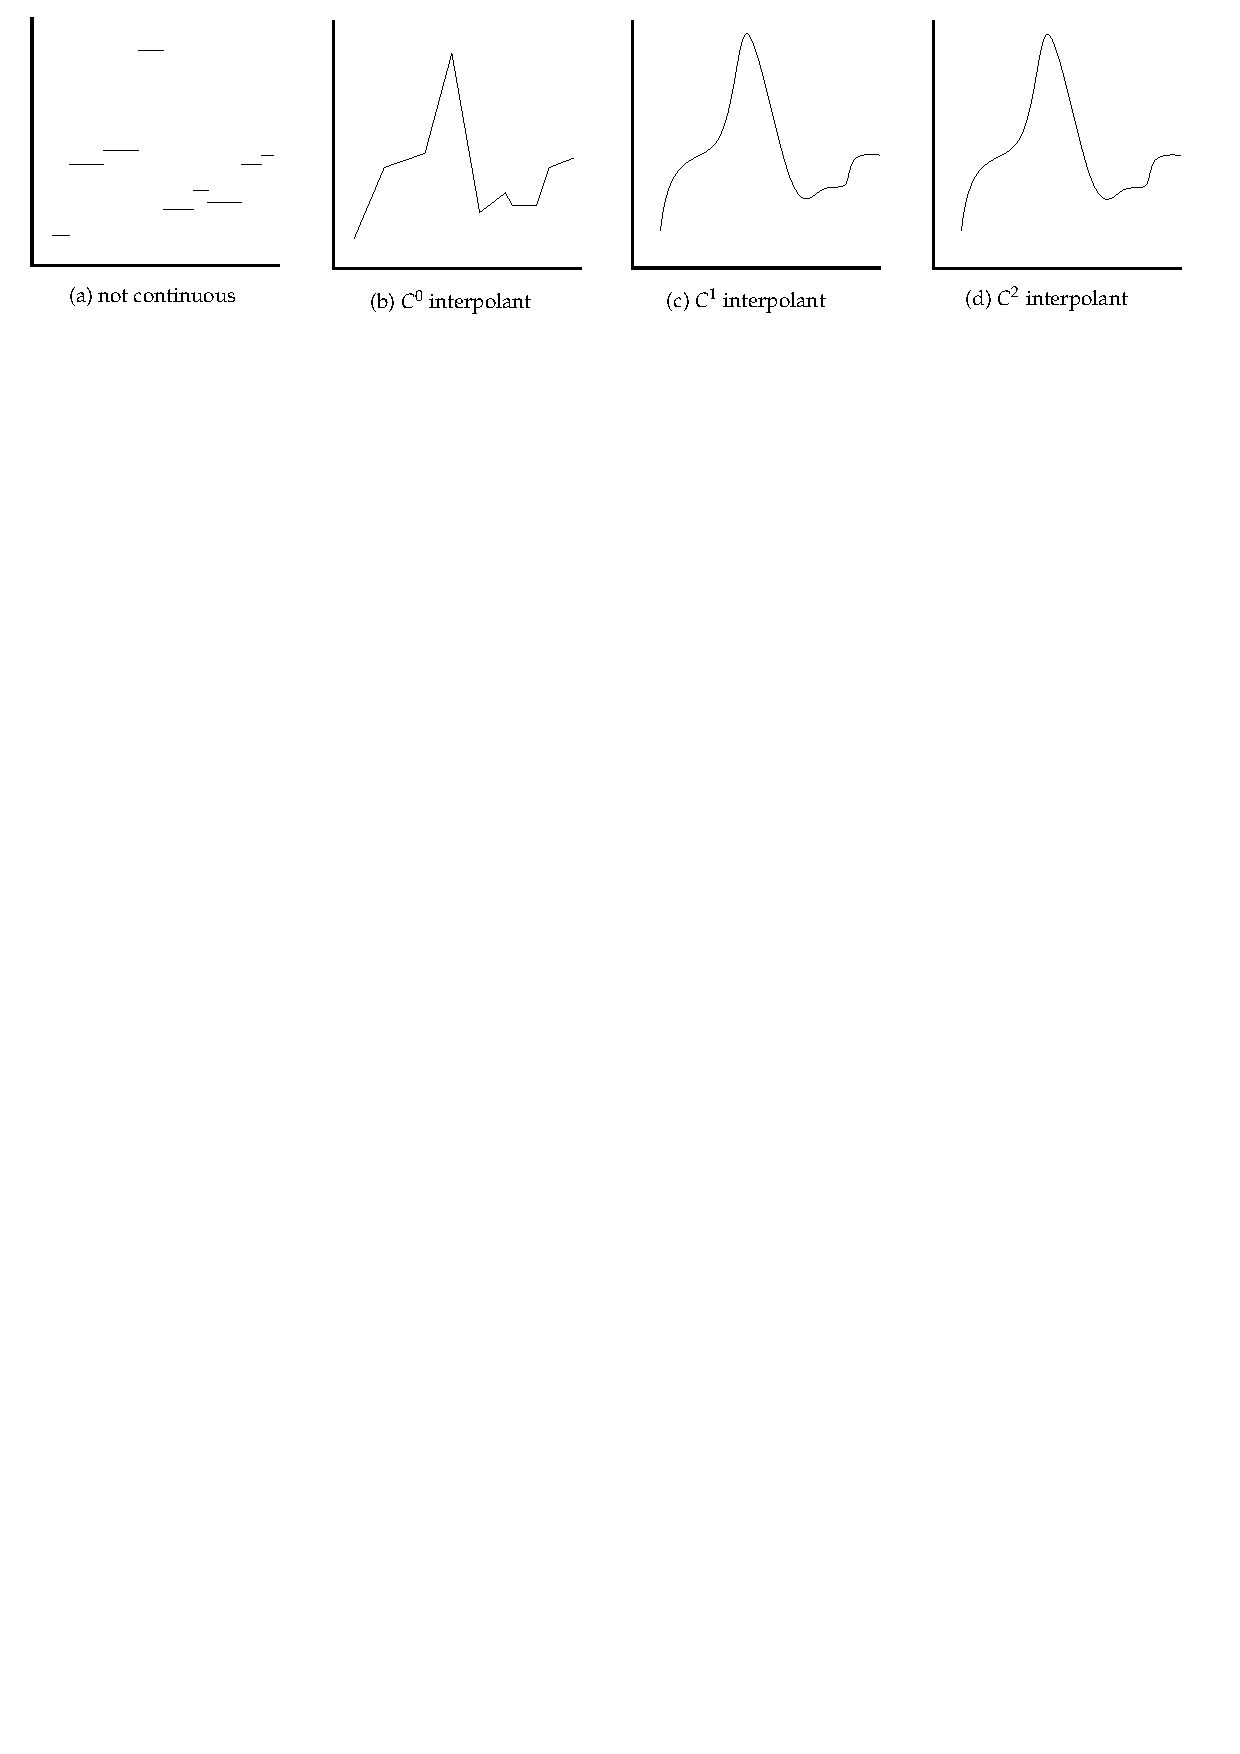
\includegraphics[width=0.9\linewidth]{figs/continuity}
  \caption{$C^0$ interpolant is a function that is continuous but the first derivative is not possible at certain locations; $C^1$ interpolant has its first derivative possible everywhere; $C^2$ interpolant has its second derivative possible everywhere (this one is more difficult to draw).}
\label{fig:continuity}
\end{figure}



%-------------------------------------------
%-
\section{Fitting polynomials}


%%%
%
\subsection{One global function}

We know that if we have $n$ points in $S$ in in $\mathbb{R}^3$ (the samples are lifted to their elevation), there is one polynomial of degree at most $n-1$.

This interpolant will be exact, continuous and smooth (at least $C^2$).
However, it will not be local (which is problematic for terrains), and finding the polynomial of a high degree for large datasets might be impossible (or take a lot of time).

The biggest concern polynomials is probably that while the interpolant is exact (the surface passes through the sample points), higher-degree polynomials can oscillate between the samples and `overshoot', \ie\ be (far) outside the minimum or maximum $z$ values of the the set $S$.
This is known as the Runge's phenomenon in numerical analysis, and is shown in Figure~\ref{fig:polynomial}.
\begin{figure}
  \centering
  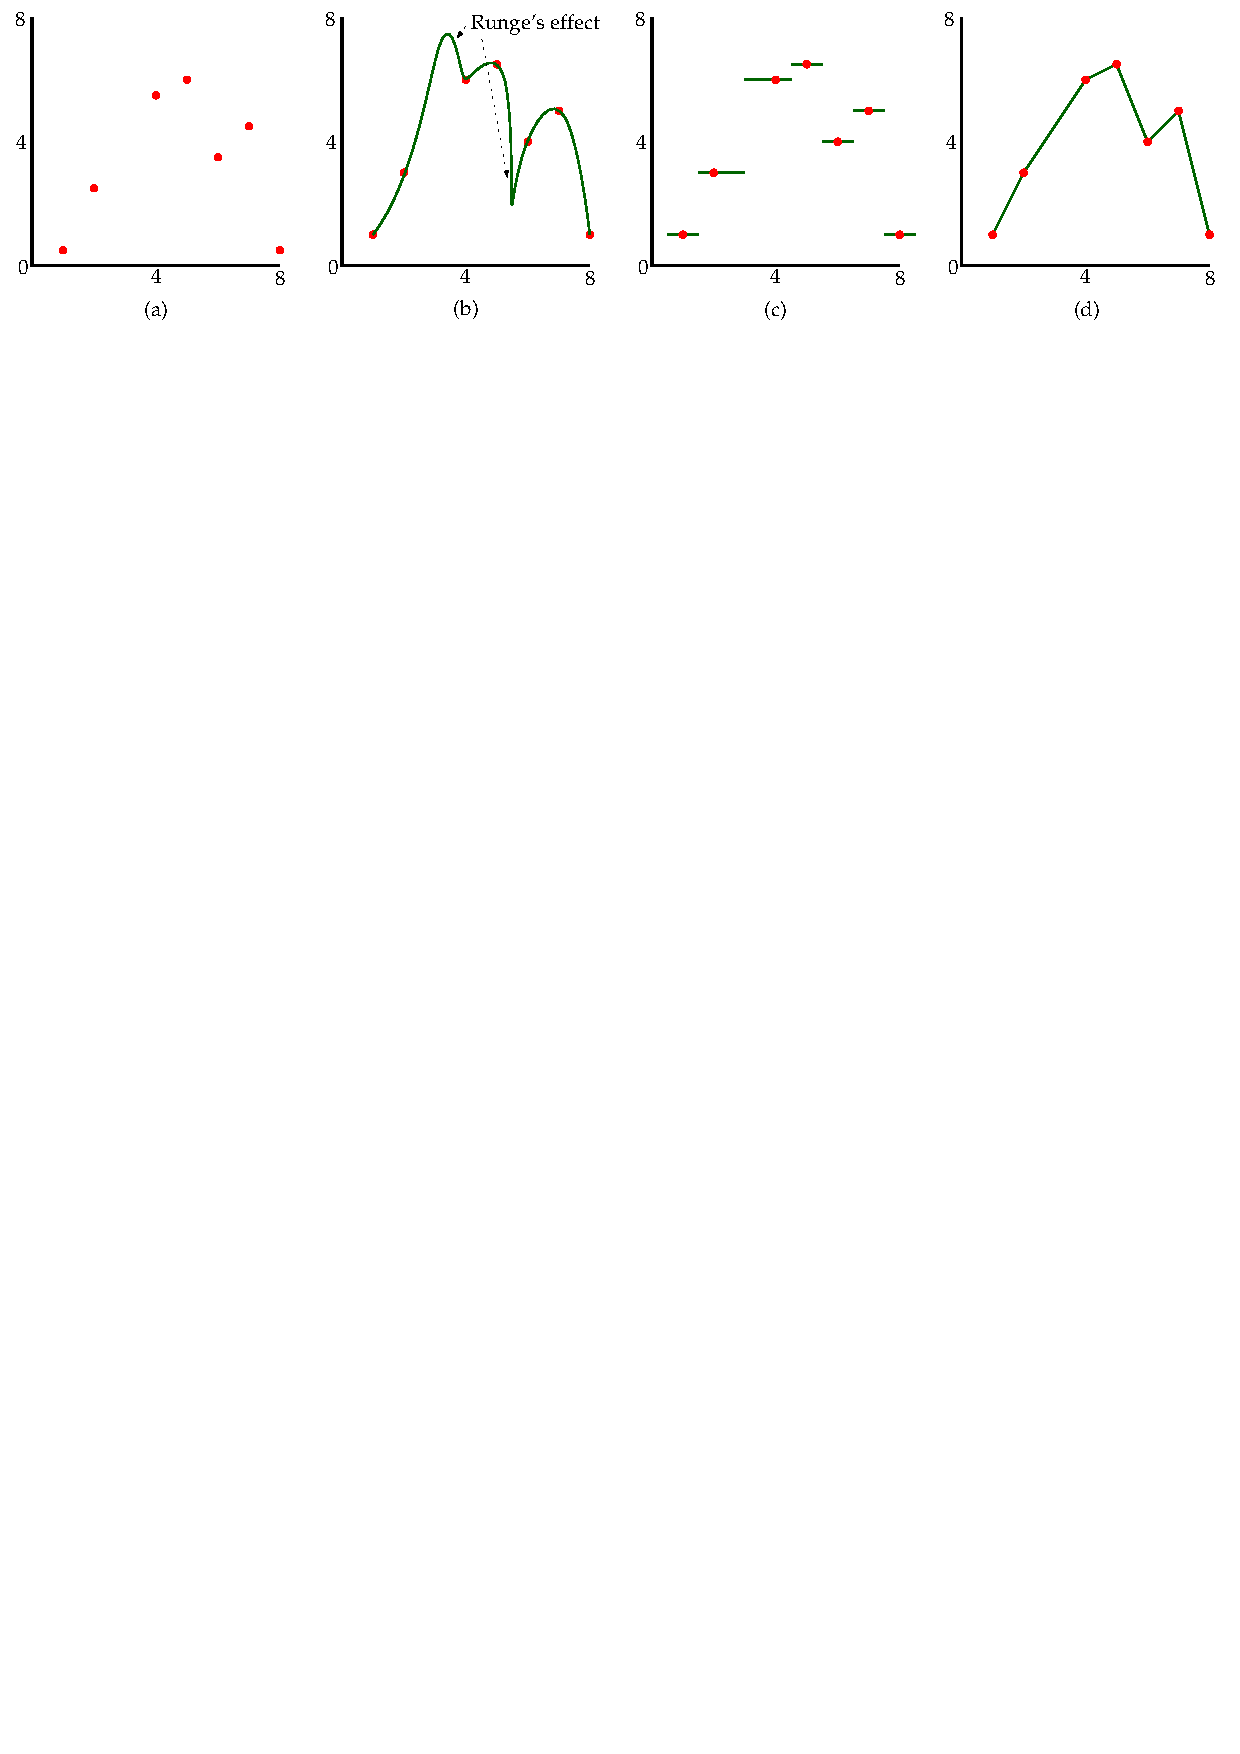
\includegraphics[width=\linewidth]{figs/polynomial}
  \caption{A few of the interpolation methods shown for a 1D dataset. \textbf{(a)} Input sample points. \textbf{(b)} Polynomial fitting, and the Runge's effect shown. \textbf{(c)} Natural neighbour. \textbf{(d)} Linear interpolation in TIN.}
\label{fig:polynomial}
\end{figure}



%%%
%
\subsection{Splines: piecewise polynomials}

Splines are piecewise polynomials, each piece is connected to its neighbouring piece in a \emph{smooth} manner: along the edges and at the data points the function is usually still $C^1$ or $C^2$ (in other words, where 2 or more polynomials connect, they have the same values for their tangents).

In practice, for terrain modelling, splines are preferred over one polynomial function because of the reasons mentioned above (mostly Runge's effect) and because computing the polynomial for large datasets is very inefficient.
The polynomials used in each piece of the subdivision is usually of low degree ($\leq 5$)

%

There are several types of splines (and variation of them, such as Bézier), and most of them are not suited for terrains.
The most used spline in practice seems to be the \emph{regularised spline with tension} (RST), where the dataset is decomposed into square pieces of a certain size.
The Runge's effect (also called \emph{overshoots}) are eliminated (since the degree is low), and the tension parameter can be tuned to obtain an interpolant that is smooth.
The method is available in the GRASS GIS\@.



%-------------------------------------------
%-
\section{Weighted-average methods}

The five interpolation methods discussed in this section are \emph{weighted-average methods}.
These are methods that use a subset of the sample points, to which a weight (importance) are assigned, to estimate the value of the dependent variable. 
The interpolation function $f$ of such methods, with which we obtain an estimation $\hat{a}$ of the dependent variable $a_i$, have the following form:
\begin{equation}
  f(x) = \hat{a_i} = \frac{\sum_{i=1}^n w_{i}(x) \, a_{i}}{\sum_{i=1}^{n} w_{i}(x)}
  \label{eq:wai}
\end{equation}
where $w_{i}(x)$ is the weight of each neighbouring data point $p_i$ (with respect to the interpolation location $x$) used in the interpolation process. 
A neighbour $p_i$ here is a sample point that is used to estimate the value of location $x$.
In the context of terrain modelling, the attribute $a$ is the elevation.


%-------------------------------------------
%-
\subsection{Nearest Neighbour Interpolation}

Nearest neigbour, or closest neighbour, is a simple interpolation method: the value of an attribute at location $x$ is simply assumed to be equal to the attribute of the nearest data point. 
This data point gets a weight of \emph{1.0}.
\begin{figure}[b]
  \centering
  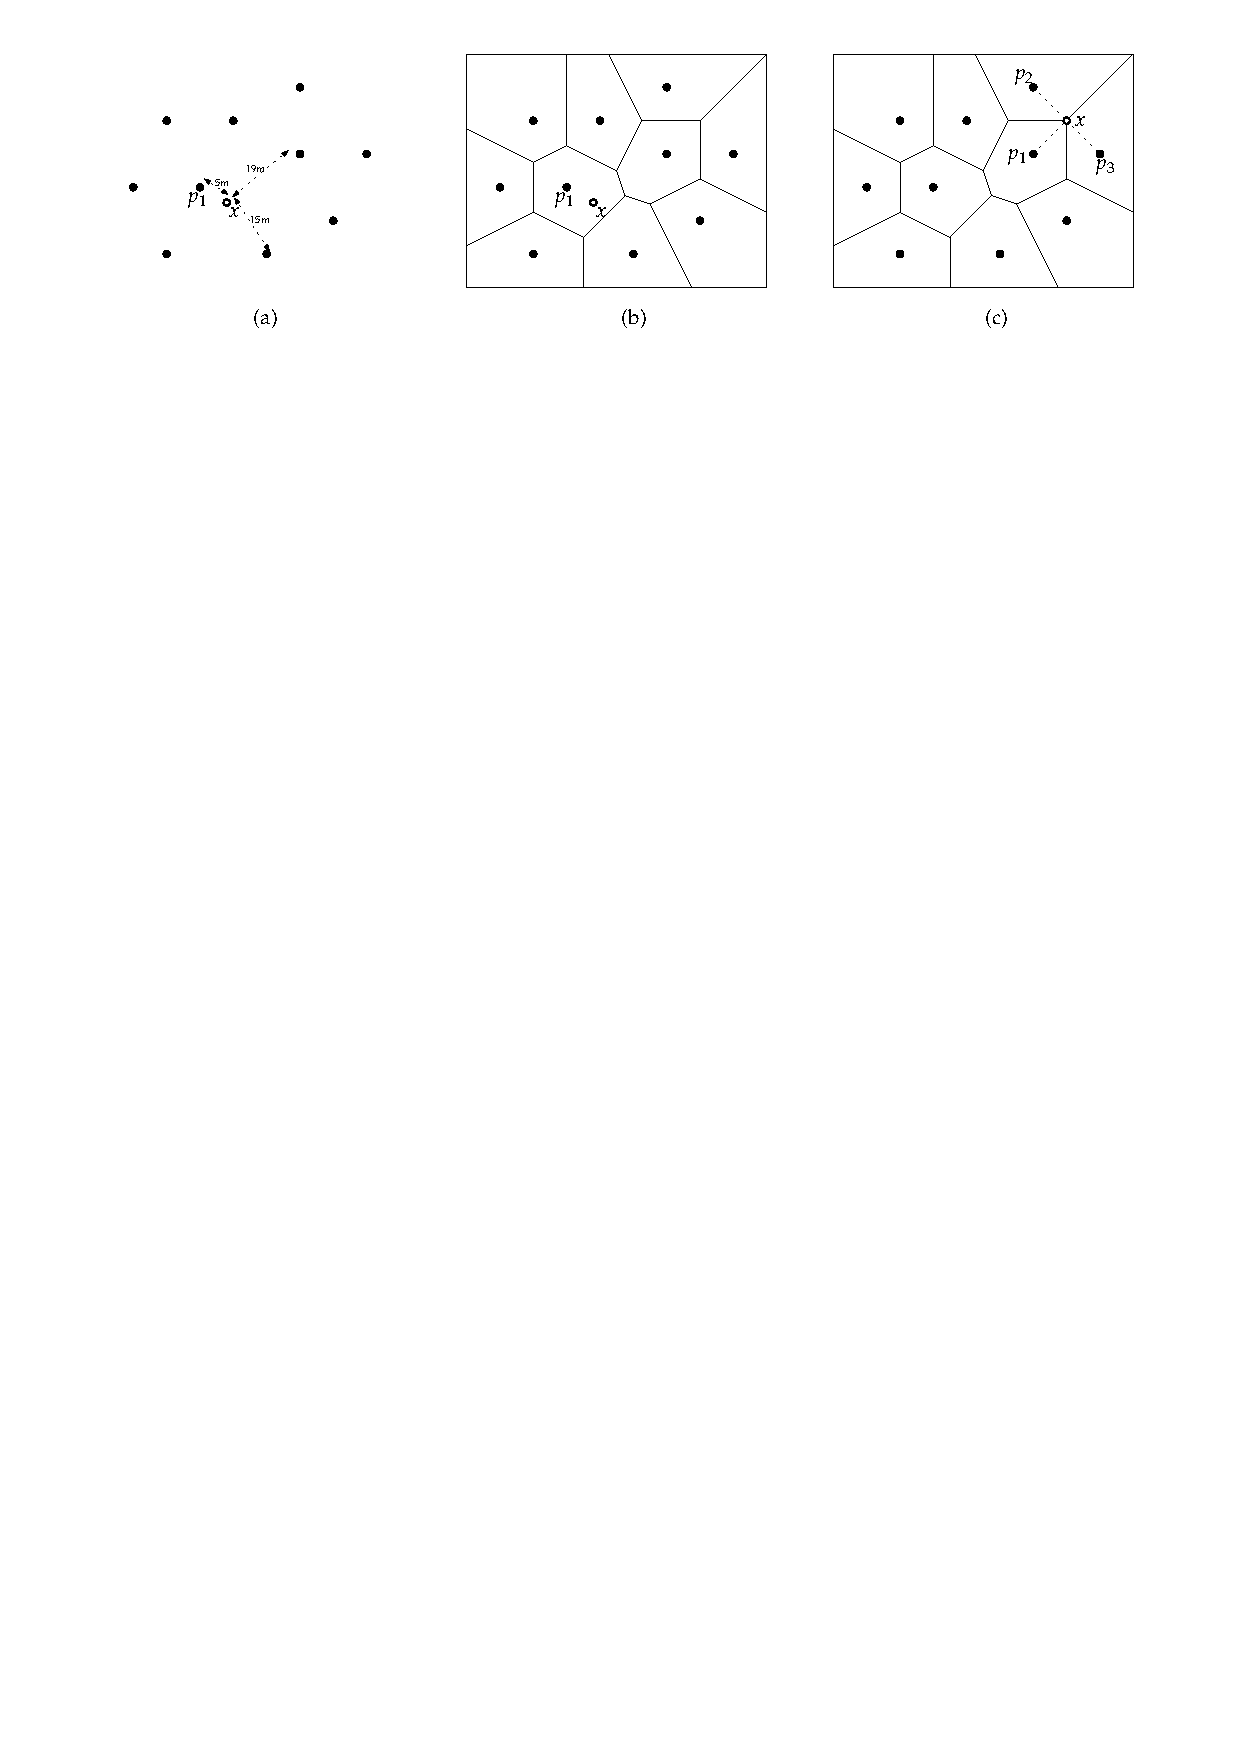
\includegraphics[width=0.95\linewidth]{figs/cn}
  \caption{\textbf{(a)} Nearest neighbour: the estimatated value at $x$ is that of the closest data point. \textbf{(b)} the Voronoi diagram can be used. \textbf{(c)} Ambiguity because $p_1$, $p_2$, and $p_3$ are equidistant from $x$; this causes discontinuities in the resulting surface.}
\label{fig:nn}
\end{figure}
Given a set $S$ of data points, if interpolation is performed with this method at many locations close to each other, the result is the Voronoi diagram (VD) of $S$, where all the points inside a Voronoi cell have the same value.

Although the method possesses many of the desirable properties (it is exact, local and can handle anisotropic data distributions), the reconstruction of continuous fields can not realistically be done using it since it fails lamentably properties 2 and 3. 
The interpolation function is indeed discontinuous at the border of cells; if the location $x$ is directly on an edge or vertex of the VD($S$), then which value should be returned?
% It is nevertheless the perfect method for reconstructing discrete fields, and is also often used in remote sensing to avoid averaging or blurring the resulting image.


%-------------------------------------------
%-
\subsection{Inverse distance weighting (IDW)}

Inverse distance weighting (IDW)---also called inverse distance to a power, or distance-based methods---is a family of interpolation methods using distance to identify the neighbours used, and to assign them weights.
IDW is probably the most known interpolation method and it is widely used in many disciplines.
As shown in Figure~\ref{fig:idw}a,
\begin{figure}
  \centering
  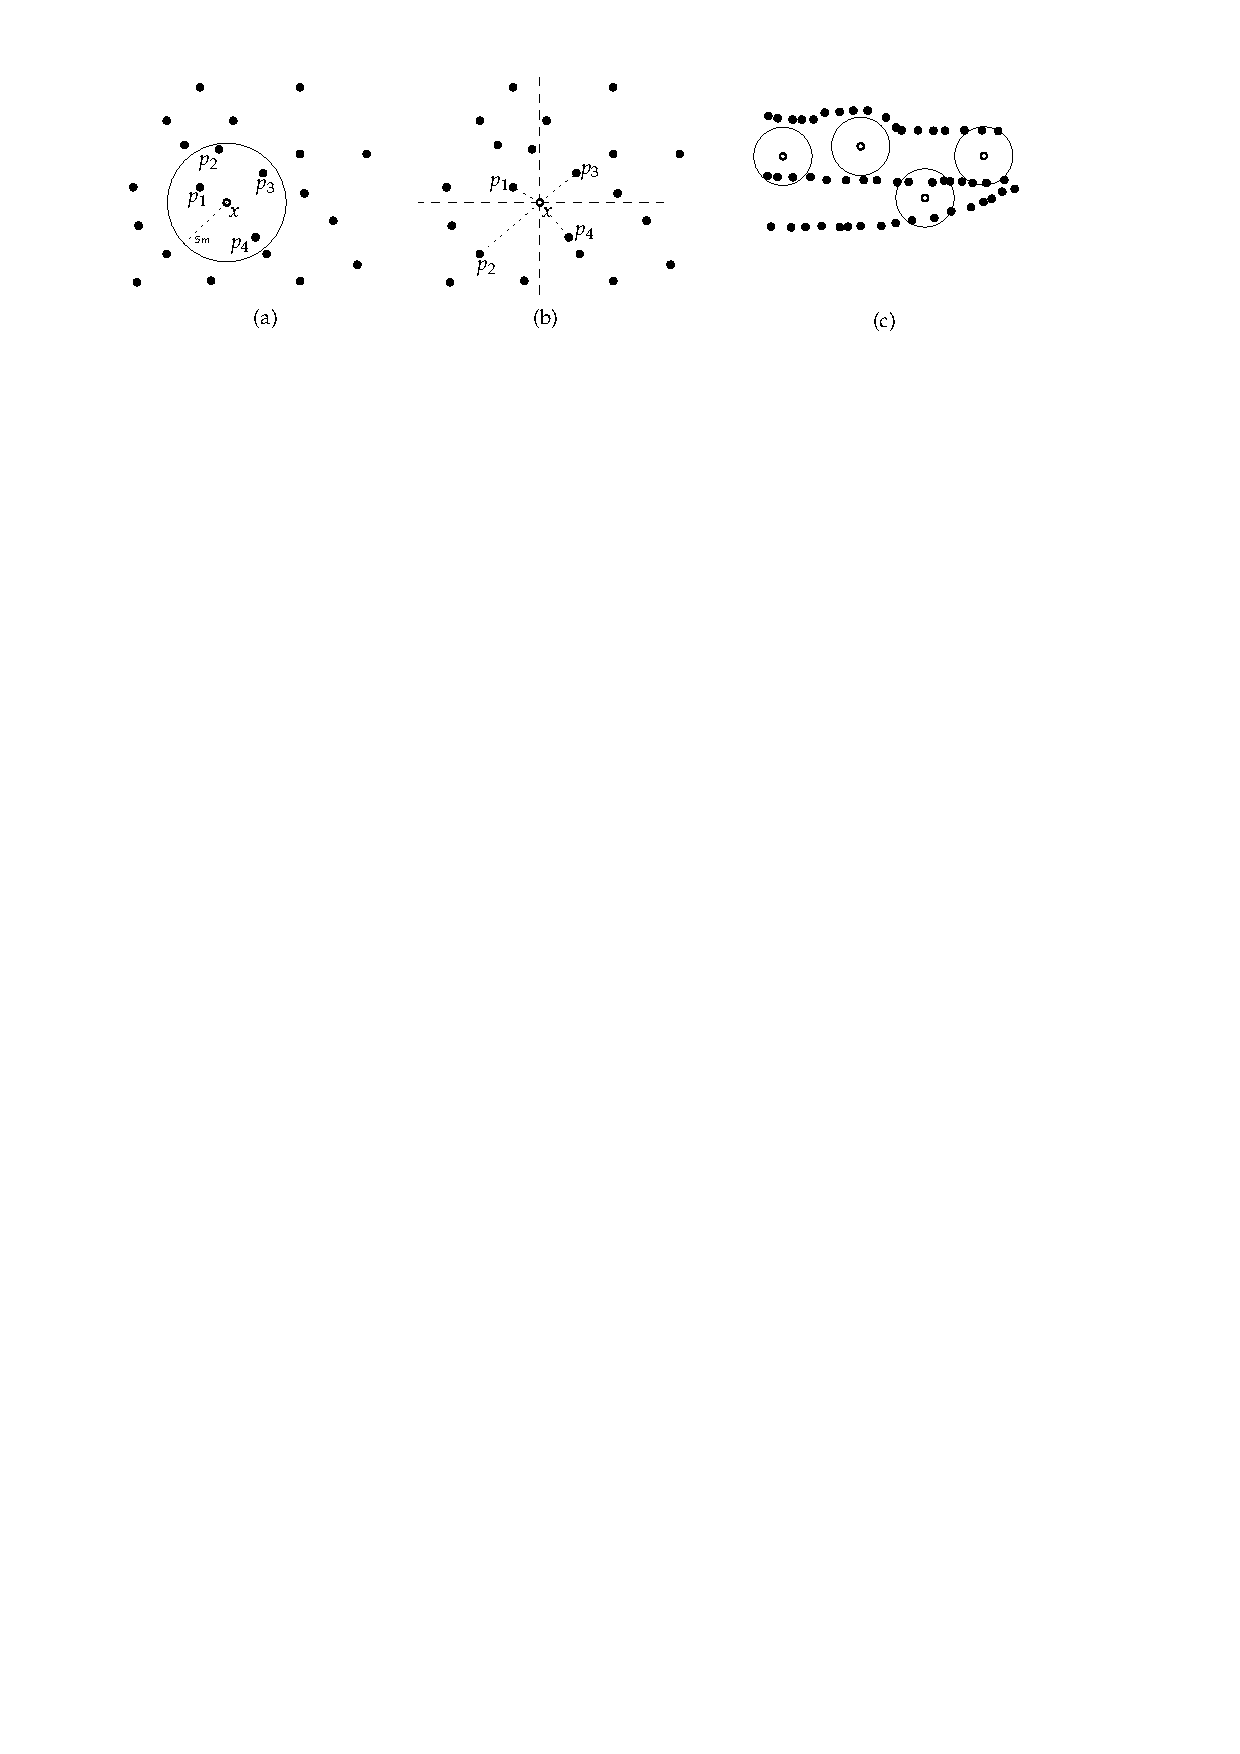
\includegraphics[width=0.95\textwidth]{figs/idw}
  \caption{\textbf{(a)} IDW interpolation with a searching circle, and the weight assigned to each neighbour used in the estimation. \textbf{(b)} IDW by choosing the closest neighbour in each quadrant. \textbf{(c)} It has (serious) problems with datasets whose distribution of samples is anisotropic.} 
\label{fig:idw}
\end{figure}
in two dimensions it often uses a `searching circle', whose radius is user-defined, to select the data points $p_i$ involved in the interpolation at location $x$. 
It is also possible to select for instance the 10 or 15 closest data points, or do that according to certain directions (\ie\ you can select for example 3 data points in each quadrant; Figure~\ref{fig:idw}b shows the case where the closest in each quadrant is used). 

The weight $w_i(x)$ assigned to each $p_i$ for a location $x$ is:
\begin{equation}
w_i(x) = |xp_i|^{-h}
\end{equation}
where $h$ defines the power to be used, and $|ab|$ is the distance between $a$ and $b$.
The power $h$ is typically 2, but other weights, such as 3, can also be used.
A very high power, say 5, will assign very little importance to points that are far away.

It should be emphasised that the size of the radius of the searching circle influences greatly the result of the interpolation: a very big radius means that the resulting surface will be smooth or `flattened'; on the other hand, a radius that is too small might have dramatic consequences if for example no data points are inside the circle (Figure~\ref{fig:idw}c shows one example).
A good knowledge of the dataset is thus required to select this parameter. 

This method has many flaws when the data distribution varies greatly in one dataset because a fixed-radius circle will not necessarily be appropriate everywhere in the data\-set. 
Figure~\ref{fig:idw}c shows one example where one circle, when used with a dataset extracted from contour lines, clearly gives erroneous results at some locations. 
The major problem with the method comes from the fact that the criterion, for both selecting data points and assigning them a weight, is one-dimensional and therefore does not take into account the spatial distribution of the data points close to the interpolation location.

IDW is exact, local, and can be implemented in an efficient manner.
However, as mentioned above, there are cases where is might not be continuous (nor smooth), it suffers from the distribution of sample points, and we cannot claim that it is automatic since finding the correct parameters for the search radius is usually a trial-and-error task.
If the closest data points in each quadrant are used, then the method can be made automatic and continuous.


%-------------------------------------------
%-
\subsection{Linear Interpolation in a TIN}

This method is popular for terrain modelling applications and is based on a triangulation of the data points. 
As is the case for the VD, a triangulation is a piecewise subdivision (tessellation) of the plane, and in the context of interpolation a linear function is assigned to each piece (each triangle). 
Interpolating at location $x$ means first finding inside which triangle $x$ lies, and then the height is estimated by linear interpolation on the 3D plane defined by the three vertices forming the triangle (the samples are lifted to their elevation value). 
The number of samples used in the interpolation is therefore always 3, and their weight is based on the barycentric value (see below).
To obtain satisfactory results, this method is usually used in 2D with a Delaunay triangulation because, among all the possible triangulations of a set of points in the plane, it maximizes the minimum angle of each triangle. 

The method is exact, continuous, local, adaptative, efficient, and automatic.
Only the property \#3 is not fulfilled (at the edges of the triangles).


%%%
\paragraph{Data-dependent triangulations.}
It was shown in Chapter~\ref{chap:dtvd} and in \reffig{fig:whydt} that, for terrain modelling, the Delaunay triangulation is preferred over other triangulations because it favours triangles that are as equilateral as possible.
However, it should be noticed that the elevation of the vertices are not taken into account to obtain the DT, \ie\ if we changed the elevation of the samples we would always get the same triangulation.
One might therefore wonder whether the DT best approximates the morphology of a terrain.

A triangulation that considers the elevation (or any $z$ coordinate) is called a \emph{data-dependent triangulation}.
The idea is to define a set of criteria (instead of the empty circumcircle).
One example is trying to minimise the change in normals for the two incident triangles of an edge.
While such methods will yield longer and skinnier triangles, these might better approximate the shape of the terrain for some specific cases.
One drawback of these methods is that different criteria will be required for different cases, and that computing such triangulation can be computationally expensive.
In practice, one would need to first compute the DT, and then take each edge (and the two incident triangles), and perform a local flip based on the elevation values; the final triangulation is obtained by optimisation the wished criterion.



%%%
\paragraph{Barycentric coordinates.}
\begin{figure}
  \centering
  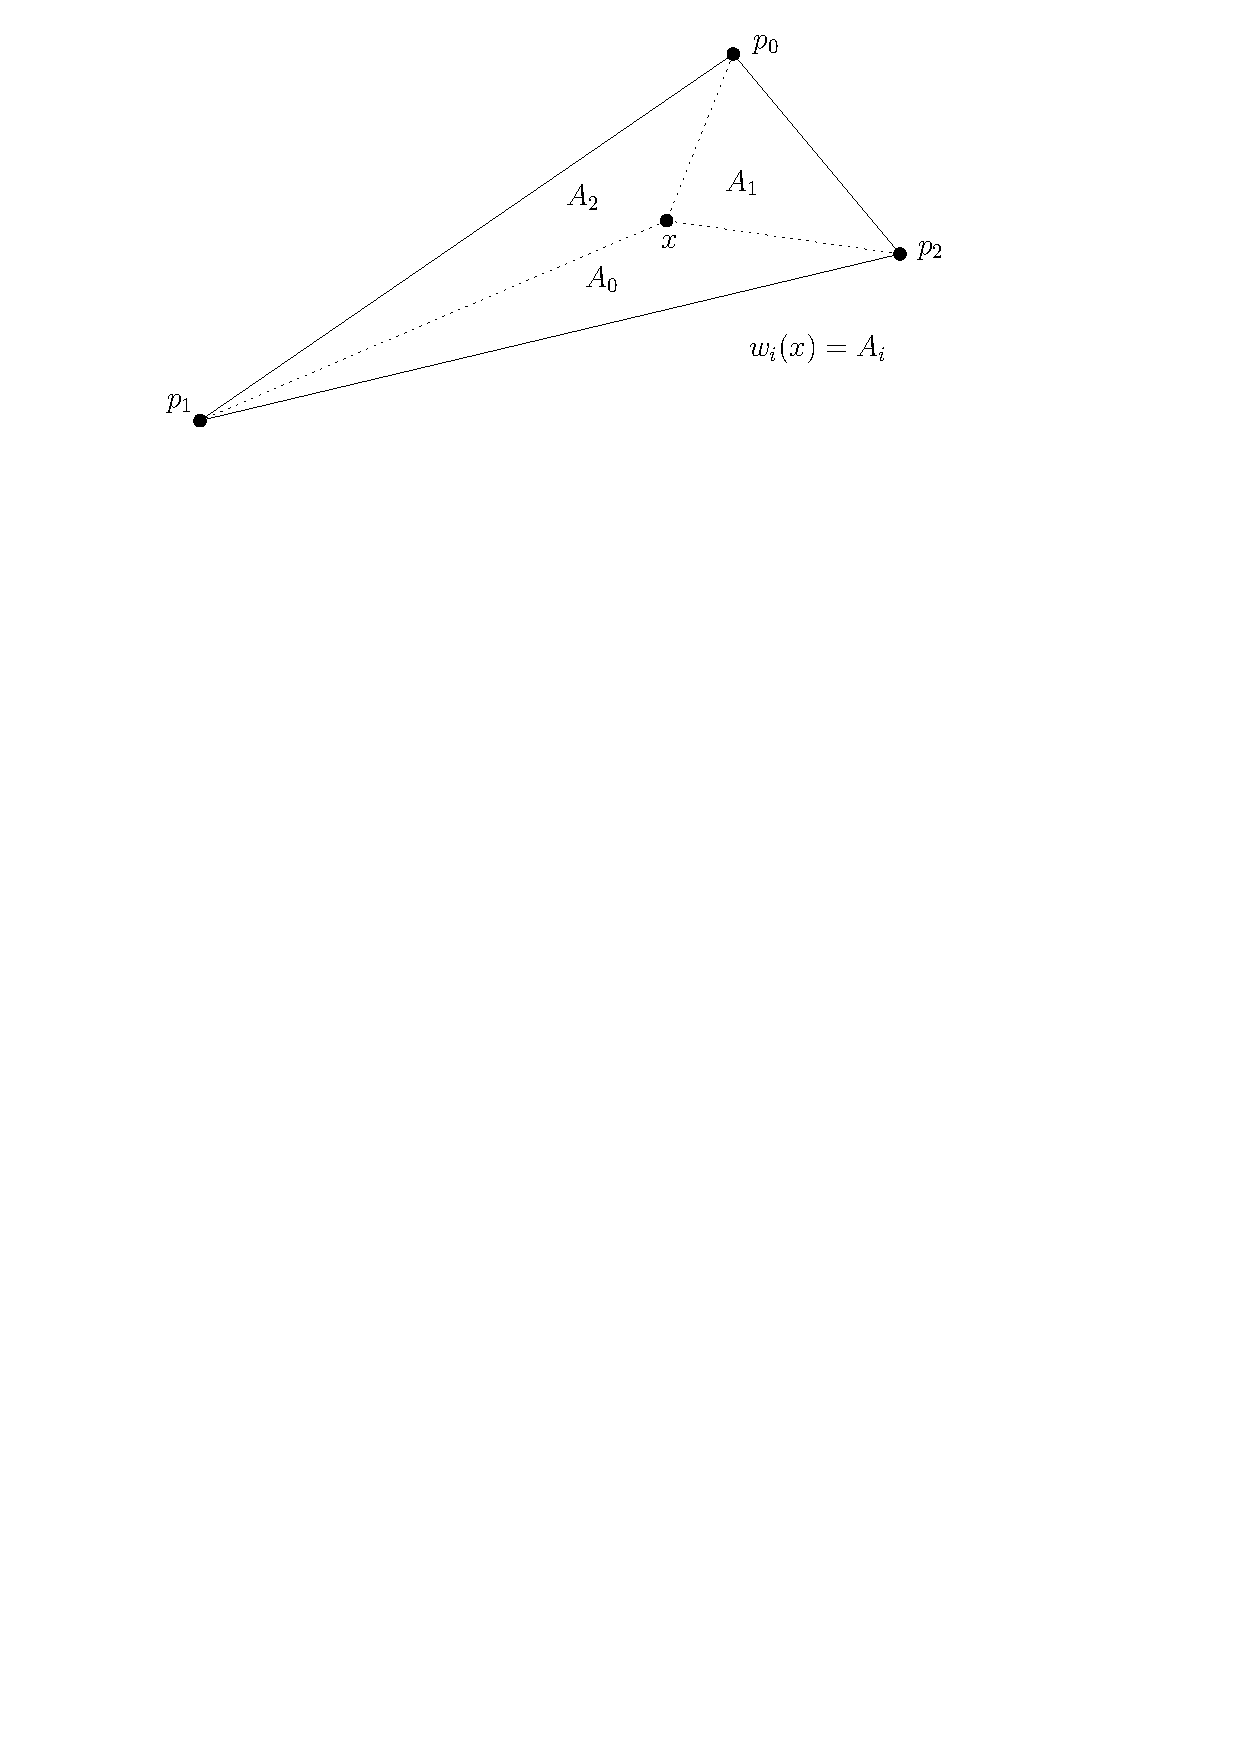
\includegraphics[width=0.5\textwidth]{figs/li}
  \caption{Barycentric coordinates. $A_i$ defines the area of a triangle.} 
\label{fig:li}
\end{figure}
The linear interpolation in a triangle can be efficiently implemented by using barycentric coordinates, which are local coordinates defined within a triangle.
Referring to Figure~\ref{fig:li}, any point $x$ inside a triangle $p_1p_2p_3$ can be represented as a linear combination of the 3 vertices:
\[
  x = w_0p_0 + w_1p_1 + w_2p_2
\]
and 
\[
  w_0 + w_1 + w_2 = 1   
\]
The coefficients $u_i$ are the barycentric coordinates of the point $x$ with respect to the triangle $p_1p_2p_3$.
Finding the coefficients $w_0$, $w_1$, and $w_2$ can be done by solving a system of linear equations.
If we subtract $p_2$ from $x$, and we use $w_2 = 1 - w_0 - w_1$, we obtain
\[
  x - p_2 = w_0(p_0-p_2) + w_1(p_1 - p_2)
\]
We obtain 2 vectors ($p_0-p_2$ and $p_1-p_2$), which represent 2 edges of the triangle.
This equation can be solved and we find that the 3 coefficients are equal of the area of the 3 triangle subdividing the original triangle (as shown in Figure~\ref{fig:li}).


%%%
\paragraph{Higher-order function in each triangle.}
% TODO : Clough-Tocher? Since in QGIS, C^1, easy to implement. But complex to explain... probably out of scope for this course?
% http://lagrange.univ-lyon1.fr/docs/scipy/0.17.1/generated/scipy.interpolate.CloughTocher2DInterpolator.html#id4
% Very good explanation: https://www.youtube.com/watch?v=3jnySeiLkLY
% Sect.5.1 explains the same in written form...
% https://ac.els-cdn.com/0167839686900166/1-s2.0-0167839686900166-main.pdf?_tid=1c5f9067-0645-4c1c-926d-b12eb512332b&acdnat=1541412540_b04a3b4f43f16cea71969311c501e036
Notice that it is possible to modify the linear function inside each triangle by a higher-order function.
As as the case for splines, there are \emph{several} ways to achieve this, and the details of these is out of scope for this course.
These methods are usually used more for finite element analysis where the flow of a certain fluid (\eg\ wind) around or through a mechanical piece is studied.

%

Most methods would define a cubic Bézier polynomial inside each triangle (which is $C^1$), and then ensure that the function is $C^1$ along the edges and at the 3 vertices of the triangles.
To achieve this the normals of each vertex is calculated by averaging the normals of the incident triangles, and the normal along an edge is computed similarly with the 2 incident triangles.



%-------------------------------------------
%-
\subsection{Natural Neighbour Interpolation}

This is a method based on the Voronoi diagram for both selecting the data points involved in the process, and assigning them a weight.  
It uses two VDs: one for the set $S$ of data points, and another one where a point $x$ is inserted at the estimation location. 
The insertion of $x$ modifies \emph{locally} a VD($S$): the Voronoi cell $\mathcal{V}_{x}$ of $x$ `steals' some parts of some Voronoi cells of VD($S$), as shown in Figure~\ref{fig:nnc}.
\begin{figure}
  \centering
  \begin{subfigure}[b]{0.3\linewidth}
    \centering
    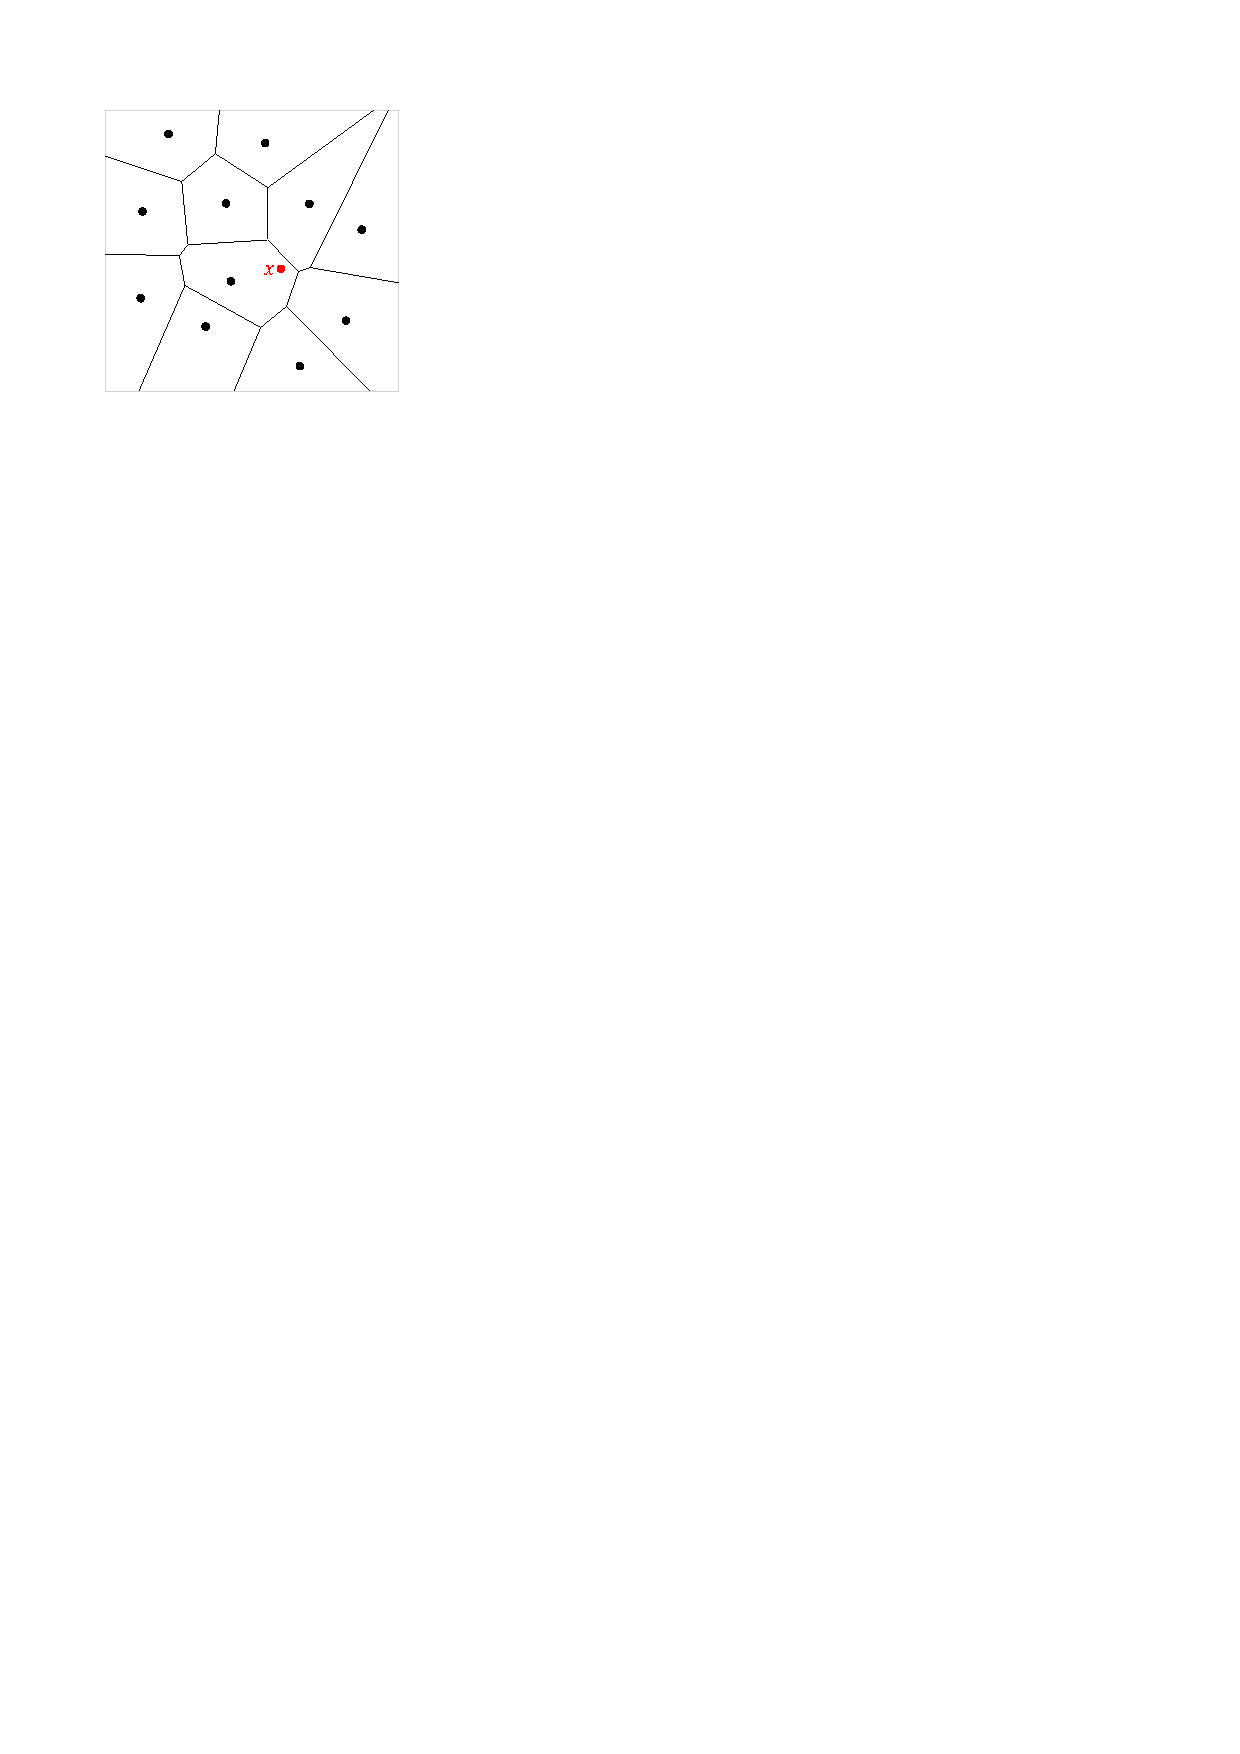
\includegraphics[width=\textwidth,page=1]{figs/laplace.pdf}
    \caption{}\label{fig:nn-a}
  \end{subfigure}%
  \begin{subfigure}[b]{0.3\linewidth}
    \centering
    \includegraphics[width=\textwidth,page=2]{figs/laplace.pdf}
    \caption{}\label{fig:nnc-a}
  \end{subfigure}
  \begin{subfigure}[b]{0.3\linewidth}
    \centering
    \includegraphics[width=\textwidth,page=3]{figs/laplace.pdf}
    \caption{}\label{fig:laplace}
  \end{subfigure}%
\caption{\textbf{(a)} The VD of a set of points with an interpolation location $x$. \textbf{(b)} Natural neighbour coordinates in 2D for $x$. The shaded polygon is $\mathcal{V}^{+}_{x}$. \textbf{(c)} The weight for the Laplace interpolant.}
\label{fig:nnc}
\end{figure}

This idea forms the basis of natural neighbour coordinates, which define quantitatively the amount $\mathcal{V}_{x}$ steals from each of its natural neighbours. 
Let $\mathcal{D}$ be the VD($S$), and $\mathcal{D}^{+} = \mathcal{D} \cup \{x\}$. 
The Voronoi cell of a point $p$ in $\mathcal{D}$ is defined by $\mathcal{V}_{p}$, and $\mathcal{V}^{+}_{p}$ is its cell in $\mathcal{D}^{+}$. 
The natural neighbour coordinate of $x$ with respect to a point $p_{i}$ is
\begin{equation}
  w_{i}(x) = \frac{Area(\mathcal{V}_{p_{i}} \, \cap \, \mathcal{V}^{+}_{x})}{Area(\mathcal{V}^{+}_{x})}
  \label{eq:nnc}
\end{equation}
where $Area(\mathcal{V}_{p_{i}})$ represents the area of $\mathcal{V}_{p_{i}}$. 
For any $x$, the value of $w_{i}(x)$ will always be between 0 and 1: 0 when $p_{i}$ is not a natural neighbour of $x$, and 1 when $x$ is exactly at the same location as $p_{i}$. 
A further important consideration is that the sum of the areas stolen from each of the $k$ natural neighbours is equal to $Area(V^{+}_{x})$, in other words:
\begin{equation}
  \sum_{i=1}^{k} w_{i}(x) = 1.
\end{equation}
Therefore, the higher the value of $w_{i}(x)$ is, the stronger is the `influence' of $p_{i}$ on $x$. 
The natural neighbour coordinates are influenced by both the distance from $x$ to $p_{i}$ and the spatial distribution of the $p_{i}$ around $x$. 

%

Natural neighbour interpolation is based on the natural neighbour coordinates. 
The points used to estimate the value of an attribute at location $x$ are the natural neighbours of $x$, and the weight of each neighbour is equal to the natural neighbour coordinate of $x$ with respect to this neighbour. 
If we consider that each data point in $S$ has an attribute $a_{i}$ (its elevation), the natural neighbour interpolation function is
\begin{equation}
  f(x) = \sum_{i=1}^{k} w_{i}(x) \, a_{i}
  \label{eq:nni}
\end{equation}
where $f(x)$ is the interpolated function value at the location $x$. 

The natural neighbour interpolant possesses all the wished properties from above, except that the first derivative is undefined at the data points. 
Its main disadvantage is that its implementation is rather complex, and obtaining an efficient one is not simple and involves complex manipulation of the VD.



%-------------------------------------------
%-
\subsection{Laplace interpolant}
\label{sec:laplace}

The Laplace interpolant, or non-Sibsonian interpolation, is a computationally faster variant of the natural neighbour interpolation method.
It is faster because no (stolen) areas need to be computed, instead the lengths of the Delaunay and the Voronoi edges are used.

%

For a given interpolation location $x$, the natural neighbours $p_i$ of $x$ are used for the Laplace interpolant.
The weight $w_i$ of a $p_i$ is obtained, as shown in the Figure~\ref{fig:laplace}, by:
\begin{equation}
  w_{i}(x) = \frac{|edge_i(\mathcal{V}^{+}_{x})|}{|xp_i|}
  \label{eq:laplace}
\end{equation}
where $|edge_i(\mathcal{V}^{+}_{x})|$ represents the length of the Voronoi edge between $x$ and $p_i$ (the orange edge in Figure~\ref{fig:laplace} for one neighbour); 
and $|xp_i|$ the Euclidean distance (in 2D) between $x$ and $p_i$ (which is the Delaunay edge).

%

If we consider that each data point in $S$ has an attribute $a_{i}$ (its elevation), the interpolation function value at $x$ is:
\begin{equation}
  f(x) = \frac{\sum_{i=1}^{k} w_{i}(x) \, a_{i}}{\sum_{i=1}^{k} w_{i}(x)}
  \label{eq:laplace2}
\end{equation}

Note that the fraction becomes indeterminate when $x$ equals one of the sample points $p_i$. 
In this case the Laplace interpolant therefore simply defines that $f(x) = a_i$.

%

Firstly the Laplace interpolant is exact: the interpolation method returns the exact value, rather than some estimate, of a sample point when it is queried at that precise location. 
Secondly, it is continuous and continuously differentiable ($C^1$) everywhere except at sites where finitely many Voronoi circles intersect. 
% We found that this is not a problem in practice.
Thirdly, it is local, \ie\ it uses only a local subset of data for the interpolation of a point. 
This limits the computational cost and supports efficient addition or removal of new data points. 
Finally, like the VD itself, it is adaptive to the spatial configuration of sample points. 
Unlike other methods such as IDW interpolation, the Laplace interpolant requires no user-defined parameters.



%-------------------------------------------
%-
\subsection{Bilinear Interpolation}

When one wants to know the value of the elevation at a location $p$, she can simply look at the value of the pixel (which is equivalent to using nearest neighbour interpolation), but this method has many drawbacks, for example when one needs to \emph{resample} a grid. 
Resampling means transforming an input grid so that the resolution and/or the orientation are different, see Figure~\ref{fig:resampling}.
\begin{figure}
  \centering
  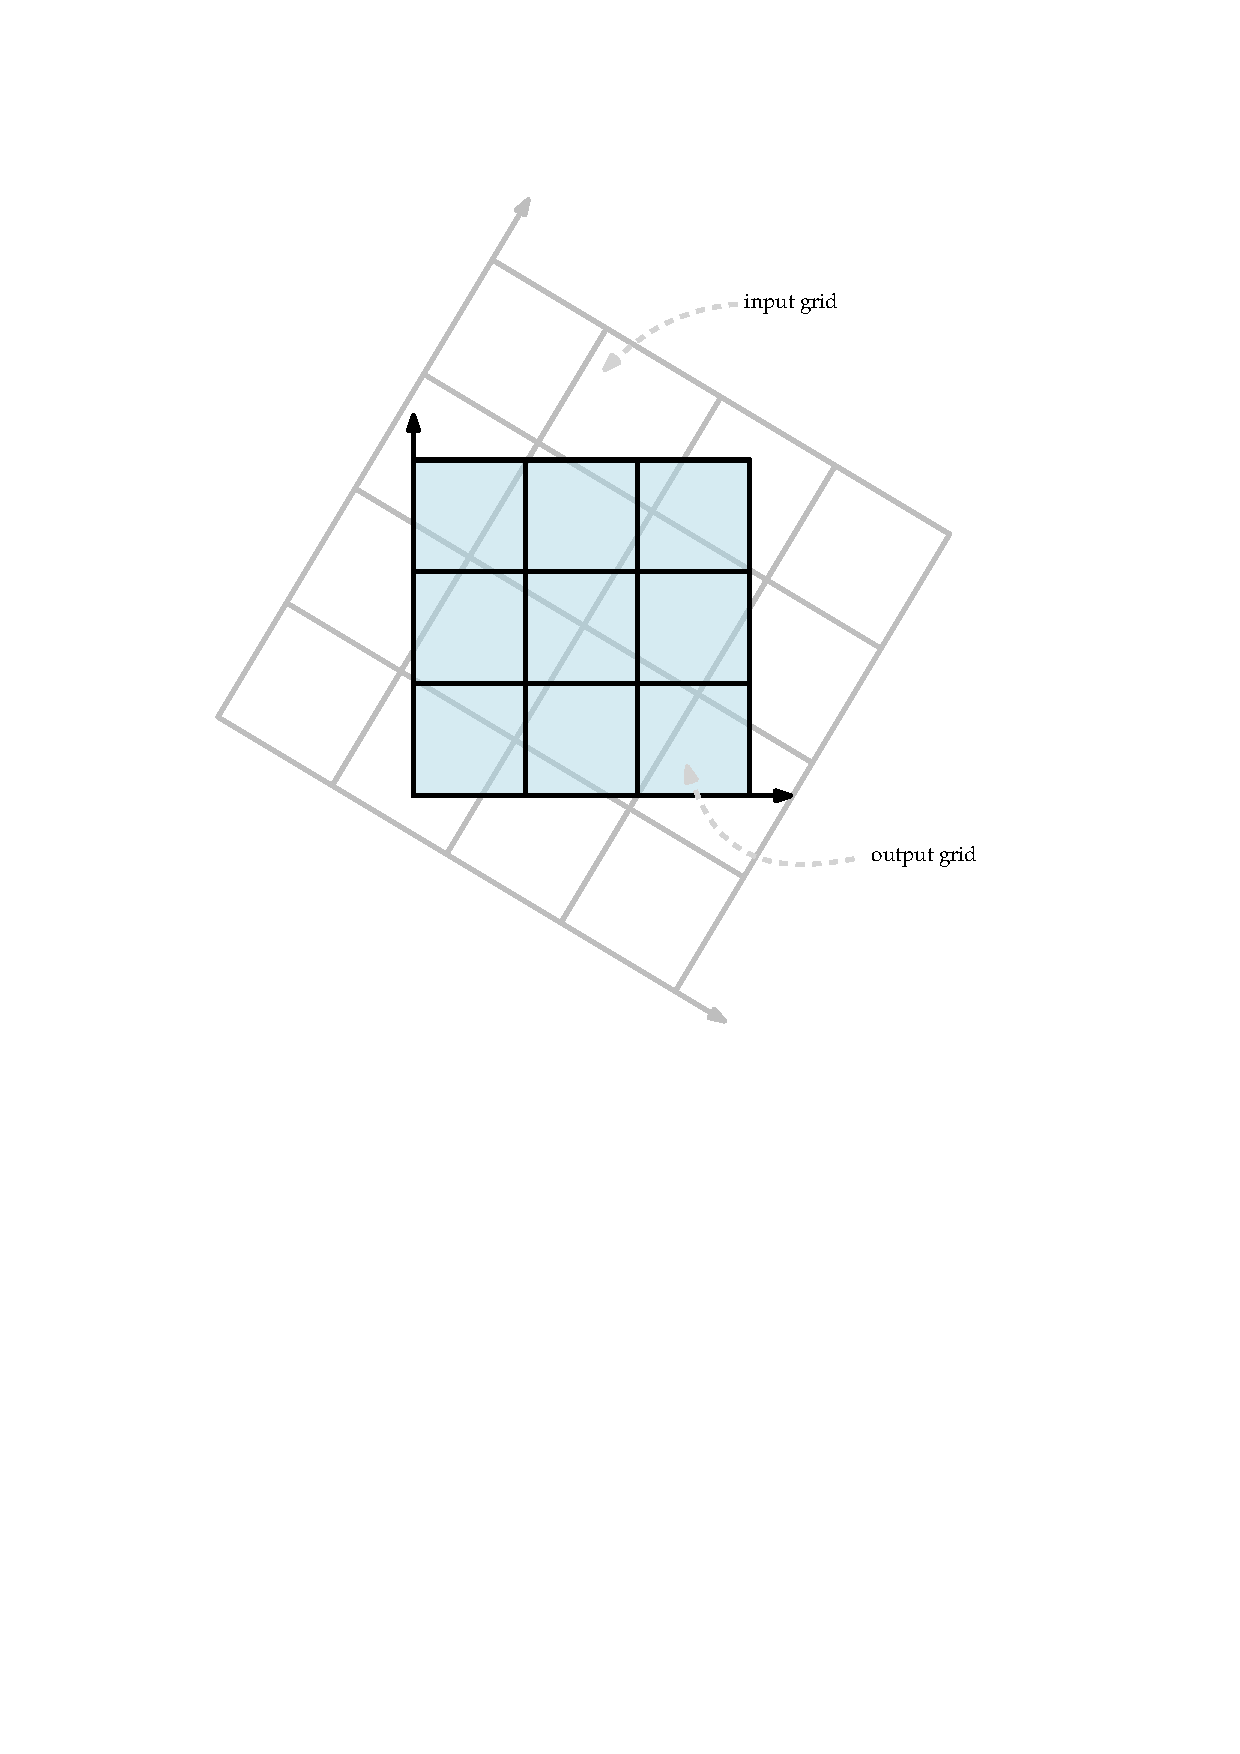
\includegraphics[width=0.4\textwidth]{figs/resampling}
  \caption{Resampling of an input grid, the output grid has different orientation.} 
\label{fig:resampling}
\end{figure}

Bilinear interpolation has been shown to give better results. 
The method, which can be seen as an ``extension' of linear interpolation for raster data, performs linear interpolation in one dimension (say along the $x$ axis), and then in the other dimension ($y$). 
Here one has to be careful about the meaning of a grid: does the value of a pixel represent the value of the whole pixel? or was the grid constructed by sampling the values at the middle of each pixel? 
In most cases, unless metadata are available, it is not known. 
But in the context of terrain modelling, we can assume that the value of a pixel represents the value at the centre of the pixel.

Suppose we have 4 adjacent pixels, each having an elevation, as in Figure~\ref{fig:bilinear}.
\begin{figure}
  \centering
  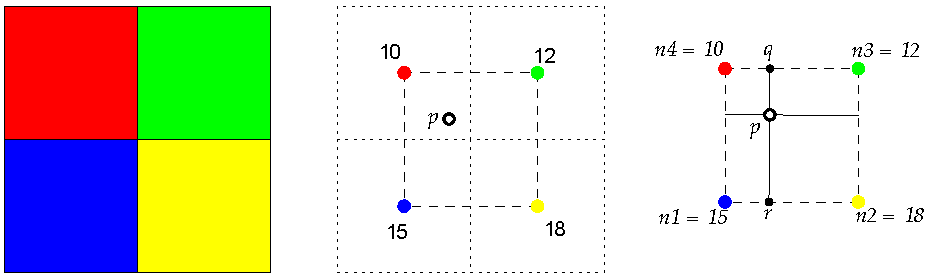
\includegraphics[width=0.9\textwidth]{figs/bilinear}
  \caption{Bilinear interpolation.} 
\label{fig:bilinear}
\end{figure}
Bilinear interpolation uses the 4 centres to perform the interpolation at location $p = (p_x, p_y)$; it is thus a weighted-average method because the 4 samples are used, and their weight is based on the linear interpolation, as explained below.
We need to linearly interpolation the values at locations $q$ and $r$ with linear interpolation, and then linearly interpolate along the $y$ axis with these values. 
% Observe that while we perform three linear interpolations, the resulting interpolant is not linear but quadratic.
Also, cotice that the result is independent of the order of interpolation: we could start with interpolating along the $y$ axis and then the $x$ axis and we would get the same result. 
For the case in Figure~\ref{fig:bilinear}, the calculation would go as follows:
\[
  \begin{array}{l}
    q_z = \frac{p_x - n4_x}{n3_x - n4_x} \times (n3_z - n4_z) + n4_z \\
   \\
    r_z = \frac{p_x - n1_x}{n2_x - n1_x} \times (n2_z - n1_z) + n1_z \\
    \\
    p_z = \frac{p_y - r_y}{q_y - r_y} * (q_z - r_z) + r_z \\
  \end{array}
\]


%%%
%
\section{Assessing the results of an interpolation method and/or fine-tuning the parameters}

Finding the ``best'' interpolation method for a given dataset, and the most suitable parameters (if any are needed), can be a rather tricky task in practice because we most often do not have extra control points.

One simple technique, which is also very easy to implement, is called \emph{jackknife}, or  cross-validation.
It is a simple statistics resampling technique to estimate the bias and the variance of an estimation.

Imagine you have a dataset $S$ consisting of $n$ sample points.
The main idea is to remove/omit from $S$ one sample point $p$ and calculate the estimation $\hat{a}_p$  obtained for the elevation at the location ($x,y$) of $p$, and to compare this value with the real value of $p$ ($a_p$).
And then to repeat this for each of the $n$ points in $S$; each estimation is thus obtained with $n-1$ points.

One method (with given parameters) for a given dataset can be characterised by computing the root-mean-square error:
\begin{equation}
  RMSE = \sqrt{\frac{\sum_{i=1}^{n}(\hat{z}_i - z_i)^2}{n}}
\end{equation}

And it is a good idea to plot the results to observe where the largest differences between the estimation and the real values are obtained, this can help in idenfiying which parameters should be fine-tuned.
See for instance one example in Figure~\ref{fig:jackknife}.
\begin{figure}
  \centering
  \begin{subfigure}[b]{0.40\linewidth}
    \centering
    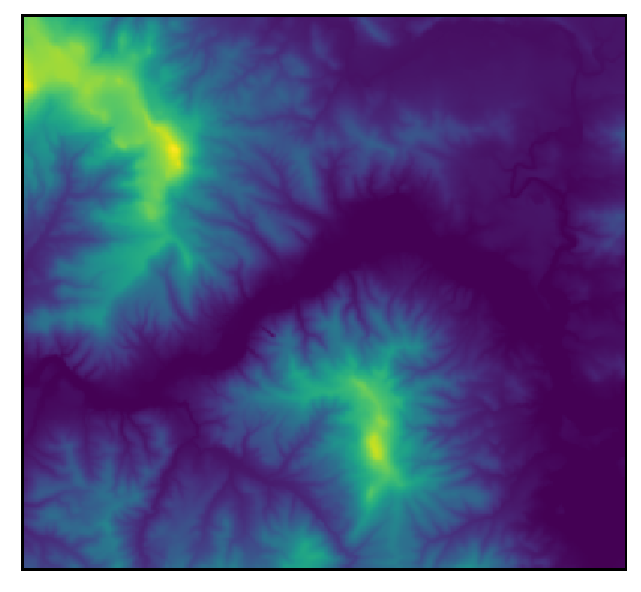
\includegraphics[width=\textwidth]{figs/jackknife/jk1.pdf}
    \caption{}
  \end{subfigure}
  \quad
  \begin{subfigure}[b]{0.475\linewidth}
    \centering
    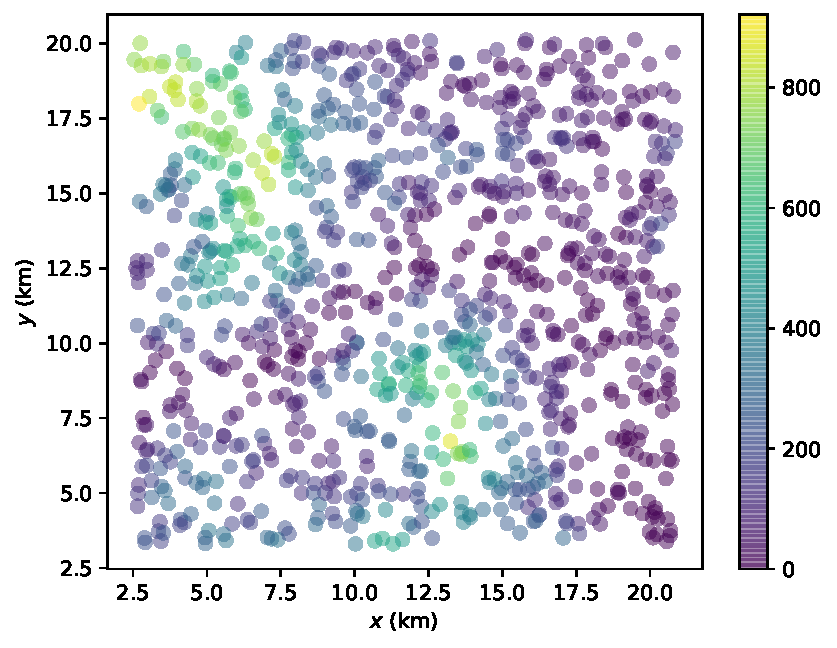
\includegraphics[width=\textwidth]{figs/jackknife/jk2.pdf}
    \caption{}
  \end{subfigure}
  \begin{subfigure}[b]{0.45\linewidth}
    \centering
    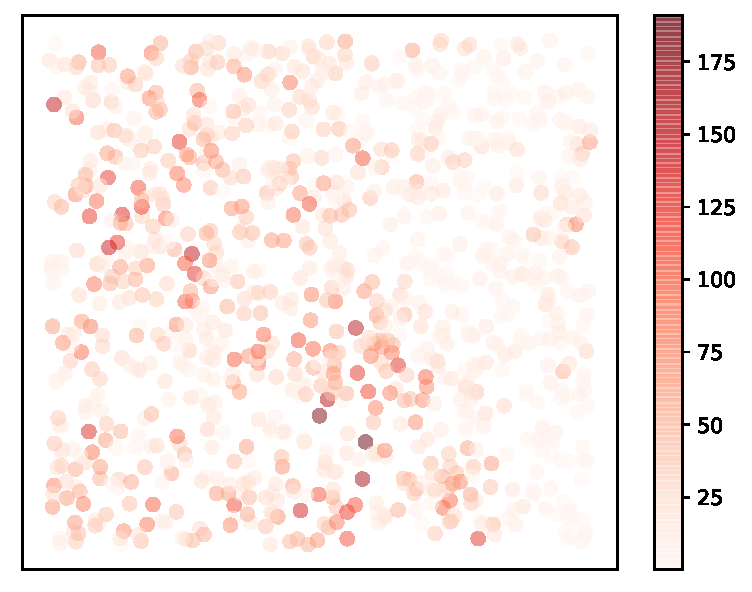
\includegraphics[width=\textwidth]{figs/jackknife/jk3.pdf}
    \caption{}
  \end{subfigure}
  \quad
  \begin{subfigure}[b]{0.45\linewidth}
    \centering
    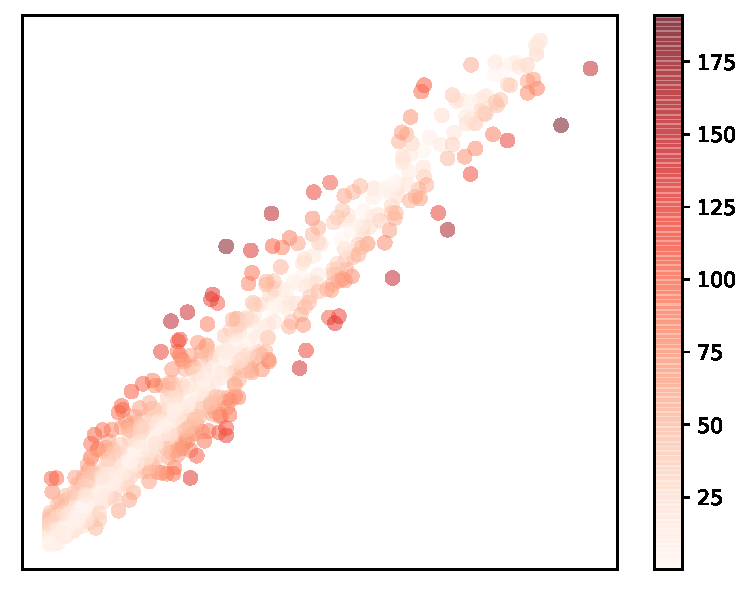
\includegraphics[width=\textwidth]{figs/jackknife/jk4.pdf}
    \caption{}
  \end{subfigure}
\caption{\textbf{(a)} A terrain of a given area containing 2 hills. \textbf{(b)} A sample of 1000 points of this terrain. \textbf{(c)} A plot of the errors (absolute values) obtained from the jackkknife (with IDW and a given search radius and power). \textbf{(d)} A plot of the absolute elevation versus the estimated ones .}
\label{fig:jackknife}
\end{figure}
It can be seen in Figure~\ref{fig:jackknife}c that the largest differences between the observed and estimated values are (mostly) concentrated around the two peaks of the terrain, which is not surprising.
The differences in the lower areas (which is water) are smaller since these areas have a flatter morphology.
Figure~\ref{fig:jackknife}d shows the same absolute differences but in a scattered plot of the observed values versus the estimated one.



%%%
%
\section{Notes and comments}


\citet{Watson92}, in his authoritative book, lists the essential properties of an `ideal' interpolation method for bivariate geoscientific datasets; we have added \emph{computationally efficient} and \emph{automatic} to the list.

\citet{Mitasova93} gives a full description of the regularised splines with tension (RST) interpolation method.
This method has also been implemented in the open-source GIS GRASS\@.

For a discussion about influence of the power in IDW on the resulting surface, please see \citet{Watson92}.

The natural neighbour interpolation method is also called Sibson's interpolation, after the name of the inventor~\citep{Sibson81}. 

To obtain a continuous interpolant even at the data points, Sibson uses the weights defined in Equation~\ref{eq:nnc} in a quadratic equation where the gradient at $x$ is considered. 
Other ways to remove the discontinuities at the data points have been proposed: \citet{Watson92} describes different methods to estimate the gradient at $x$ and how to incorporate it in Equation~\ref{eq:nni}; and \citet{Gold89} proposes to modify the weight of each $p_{i}$ with a simple hermitian polynomial so that, as $x$ approaches $p_{i}$, the derivative of $f(x)$ approaches 0. 
Modifying Equation~\ref{eq:nni} to obtain a continuous function can yield very good results in some cases, but with some datasets the resulting surface can contain unwanted effects.
Different datasets require different methods and parameters, and, for this reason, modifications should be applied with great care. 

The description of the barycentric coordinates is mostly taken from \citet{Eberly18}.

The construction of a polynomial inside each triangle of a TIN can be done with several methods. 
The simplest method is the Clough-Tocher method~\citep{Clough65,Farin85}.
It splits each triangle into 3 sub-triangles (by inserting a temporary point at the centroid of the triangle) and a cubic function is built over each.

\citet{Dyn90} shows how to obtain a data-dependent triangulation.
\citet{Rippa90} proves that the DT is the triangulation that minimizes the roughness of the resulting terrain, no matter what the actual elevation of the data is. 
Here, roughness is defined as the integral of the square of the $L^2$-norm of the gradient of the terrain.
\citet{Gudmundsson02} shows that a variation of the DT (one where $k$ vertices can be inside the circumcircle of a given triangle) can yield fewer local minima; whether it yields a ``better' terrain is an open question.


%%%
%
\section{Exercises}

\begin{enumerate}
  \item Given a triangle $\tau$ with coordinates (20.0, 72.0, 21.0), (116.0, 104.0, 32.0), and (84.0, 144.0, 26.0), estimate the elevation at $x$ = (92.0, 112.0) with linear interpolation in the triangle (both by finding the equation of the plane and with barycentric coordinates).
  \item What happens when the search distance is very large for inverse distance weighting interpolation (IDW)?
  \item For grids, can IDW or others be used instead of bilinear? If yes, how does that work?
  \item The 15 elevation samples below have been collected. You want to interpolate at two location:
  \begin{enumerate}
    \item at location ($7,6$) with IDW (radius=3; power=2); the purple circle.
    \item at location ($15,6$) with linear interpolation in TIN; the orange cross.
  \end{enumerate} 
  What are the respective answers?
  \\
  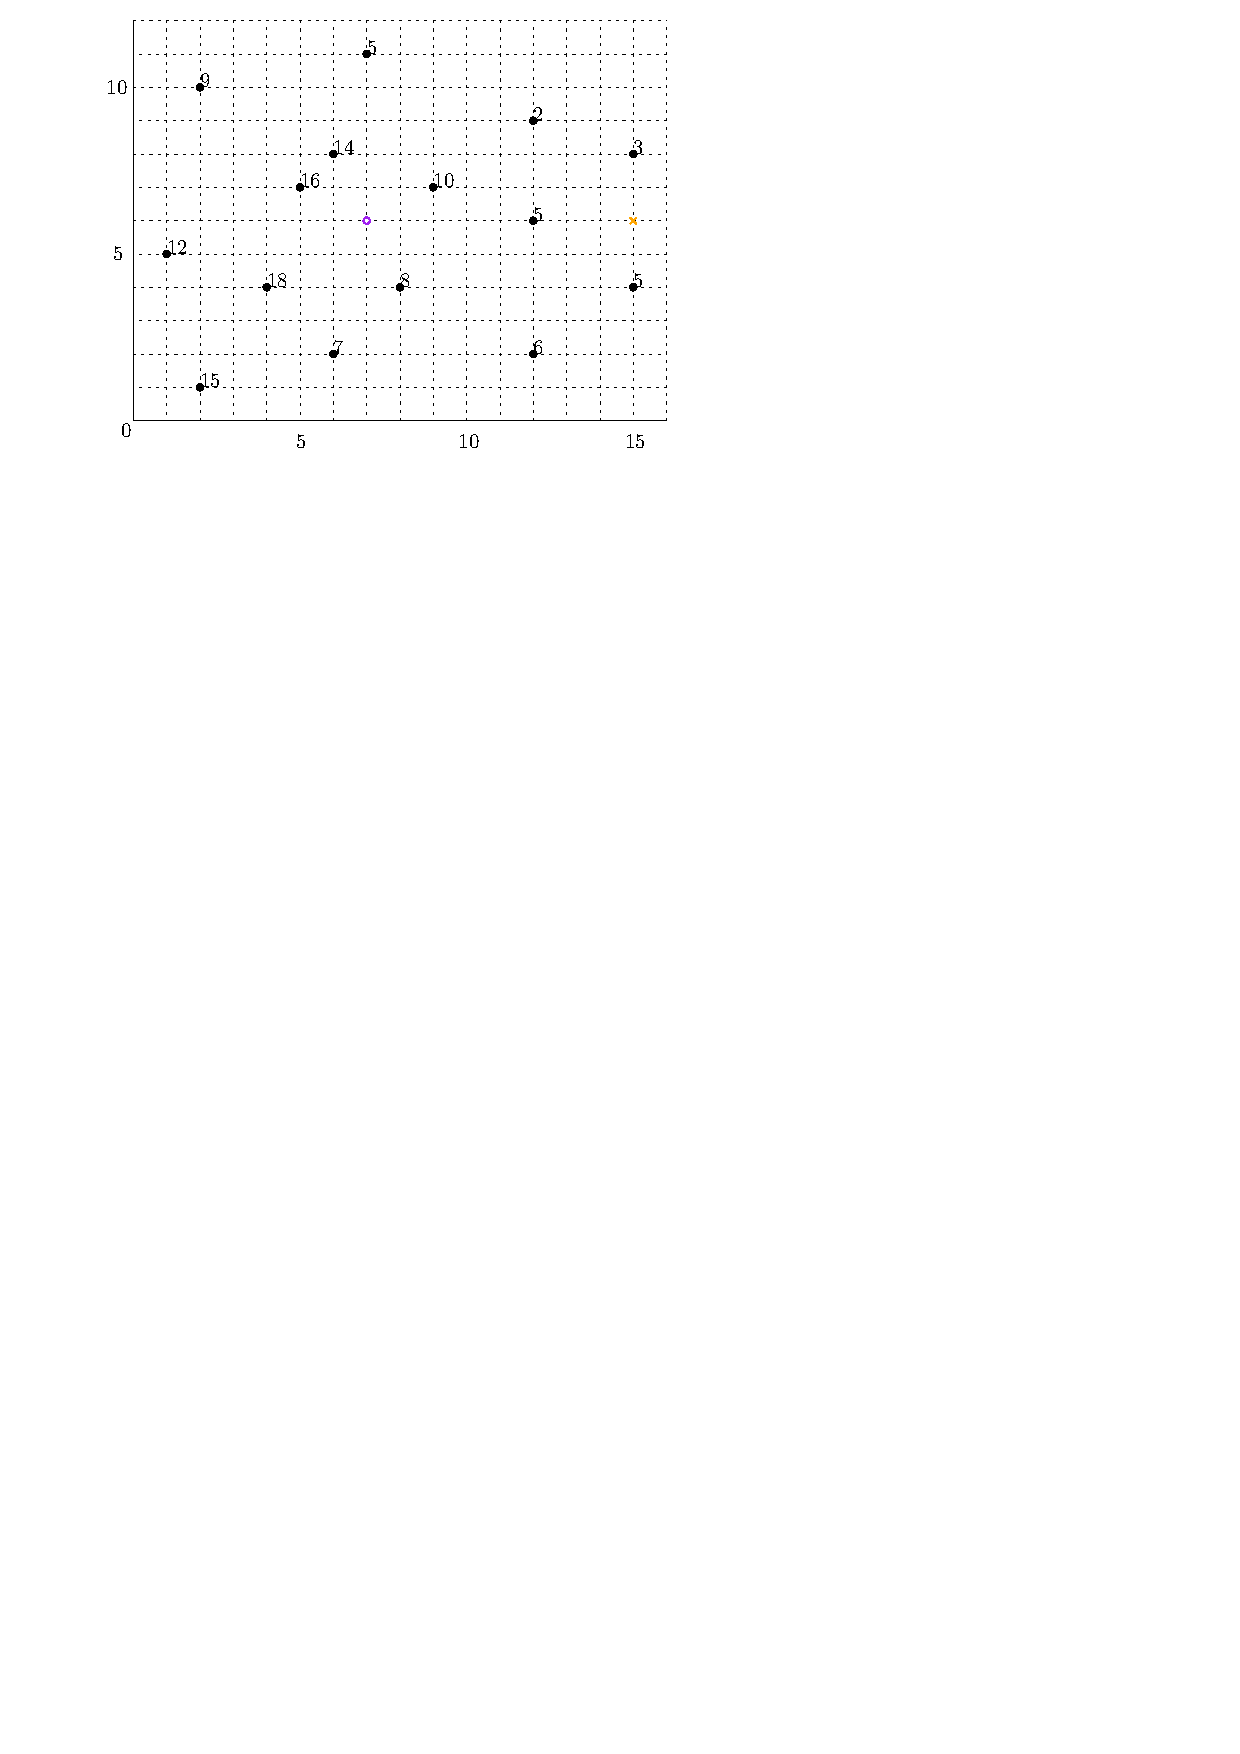
\includegraphics[width=0.75\linewidth]{figs/interpol}
\end{enumerate}
